\documentclass[12pt]{article}

%\usepackage[italian]{babel}
\usepackage[a3paper,pdftex]{geometry}
\usepackage[cm]{fullpage}

\usepackage{tikz}
\usetikzlibrary{calendar}

\newlength{\cellheight}
\setlength{\cellheight}{30mm}
\newlength{\cellwidth}
\setlength{\cellwidth}{0.14\textwidth}
\newlength{\cellsep}
\setlength{\cellsep}{2mm}
\pgfkeys{/tikz/day code =
  {
    \node (0,0) [above left,font=\Huge] {\tikzdaytext};
    \draw[rounded corners, black!50, very thick] (0,0) rectangle (-\cellwidth+\cellsep,\cellheight-\cellsep);
  }
}

\newcommand\addbithday[1]
{
    \node at (-\cellwidth+\cellsep,\cellheight-\cellsep) [below
    right,align=left, font=\tiny,black] {\color{purple} #1};
}
\newcommand\birthday
{
  % add here your birthdays...
      if (equals=01-03) {\addbithday{Mona}}
      if (equals=12-15) {\addbithday{Monica}}
}


\def\pgfcalendarmonthname#1{%
  \translate{\ifcase#1\or Gennaio
    \or Febbraio \or Marzo\or Aprile\or
    Maggio \or Giugno \or Luglio \or Augusto \or Settembre \or Ottobre\or
    Novembre \or Dicembre\fi}%
}
\begin{document}
\pagestyle{empty}
\ 

\vfill

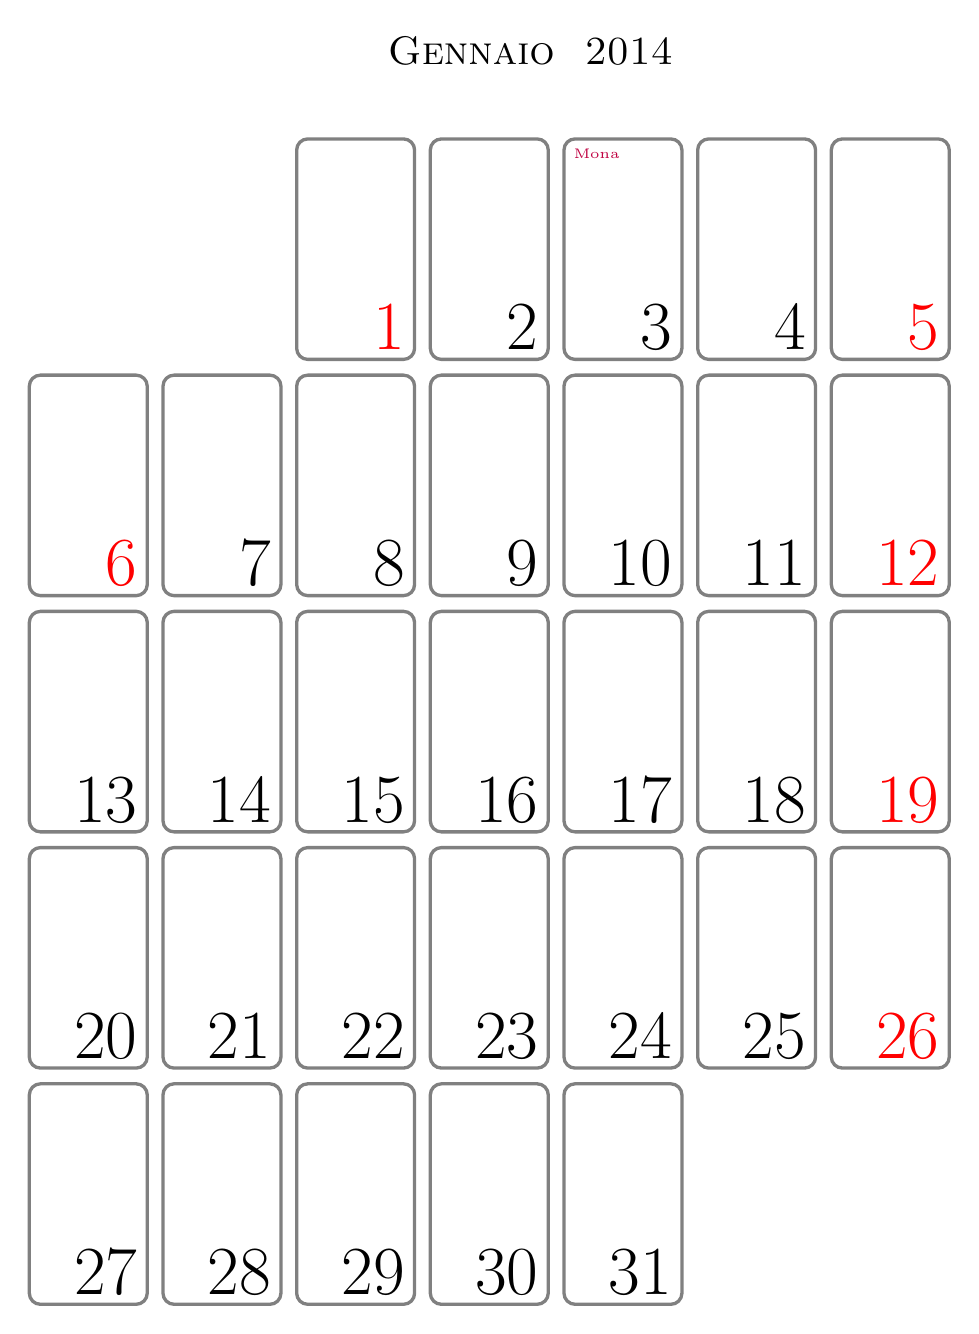
\begin{tikzpicture}
  \tikzstyle{daynode}=[
       minimum height=2.5cm,
       align=left,
       name=\pgfcalendarsuggestedname,
       every day]
  \calendar[
      dates=2014-01-01 to 2014-01-31,
      week list,
      month label above centered,
      month text=\textsc{\Large\%mt \%y0},
      day xshift=\cellwidth,
      day yshift=\cellheight,
 %     day code=\daycode
      ]
      if (Sunday,
          equals=01-01,
          equals=01-06,
          equals=05-17,
          equals=12-25,
          equals=12-26
         ) [red]
      %if (equals=01-03) {\addbithday{Mona}}
      \birthday
      ;
\end{tikzpicture}
\end{document}
